\documentclass[tikz,border=8pt]{standalone}

\usepackage{amsmath,amssymb,bm}
\usetikzlibrary{positioning, arrows.meta, shapes.geometric, fit, calc, backgrounds}

\begin{document}
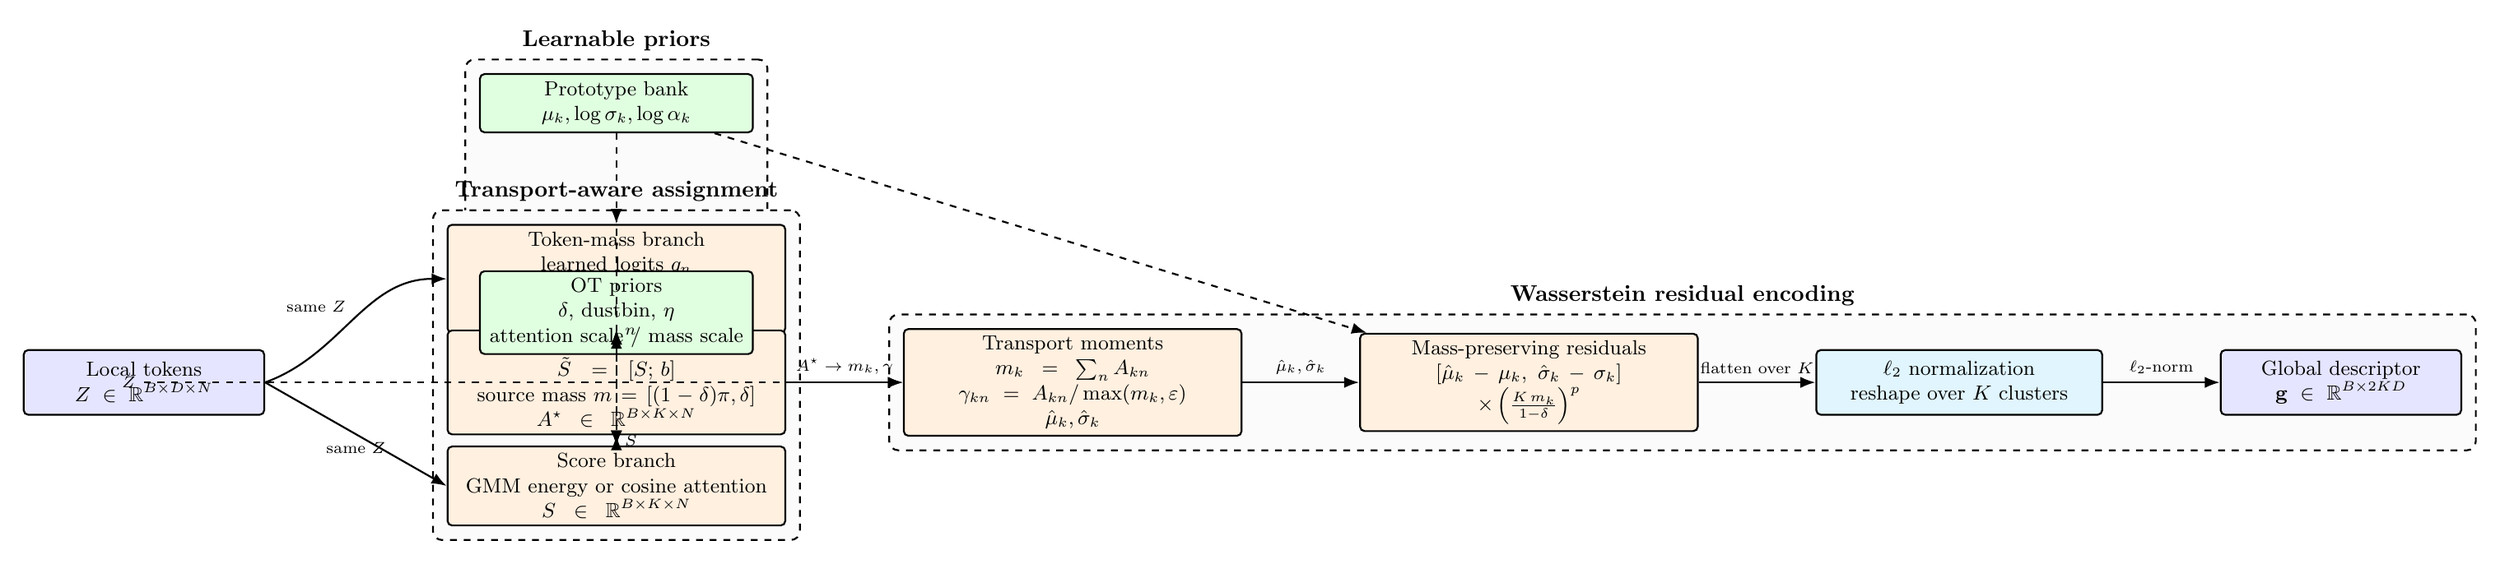
\begin{tikzpicture}[
    font=\small,
    >=Latex,
    node distance=8mm and 12mm,
    every node/.style={align=center},
    io/.style={
        draw, thick, rounded corners=2pt, fill=blue!10,
        minimum height=10mm, minimum width=35mm, text width=35mm, inner sep=3pt
    },
    module/.style={
        draw, thick, rounded corners=2pt, fill=cyan!12,
        minimum height=10mm, minimum width=42mm, text width=42mm, inner sep=3pt
    },
    mathblock/.style={
        draw, thick, rounded corners=2pt, fill=orange!12,
        minimum height=12mm, minimum width=50mm, text width=50mm, inner sep=3pt
    },
    param/.style={
        draw, thick, rounded corners=2pt, fill=green!12,
        minimum height=9mm, minimum width=40mm, text width=40mm, inner sep=3pt
    },
    group/.style={
        draw, dashed, rounded corners=4pt, thick, inner sep=6pt, fill=gray!3
    },
    flow/.style={->, thick},
    dflow/.style={->, thick, dashed},
    tiny/.style={font=\scriptsize}
]

% --------------------------------------------------------------------------
% OT-GaussVLAD operator only: token input -> transport -> residuals.
% --------------------------------------------------------------------------
\node[io] (input) {Local tokens\\$Z \in \mathbb{R}^{B\times D\times N}$};

% Parallel assignment inputs.
\node[mathblock, right=28mm of input, yshift=16mm] (mass) {Token-mass branch\\learned logits $q_n$\\or uniform $1/N$\\target mass $n=\nu/\|\nu\|_1$};
\node[mathblock, right=28mm of input] (ot) {Sinkhorn OT + dustbin\\$\tilde S=[S;\,b]$\\source mass $m=[(1-\delta)\pi,\delta]$\\$A^\star\in\mathbb{R}^{B\times K\times N}$};
\node[mathblock, right=28mm of input, yshift=-16mm] (score) {Score branch\\GMM energy or cosine attention\\$S\in\mathbb{R}^{B\times K\times N}$};

% Learnable priors.
\node[param, above=14mm of mass] (proto) {Prototype bank\\$\mu_k,\log\sigma_k,\log\alpha_k$};
\node[param, above=14mm of score] (aux) {OT priors\\$\delta$, dustbin, $\eta$\\attention scale / mass scale};

% Moment estimation and residual encoding.
\node[mathblock, right=18mm of ot] (moments) {Transport moments\\$m_k=\sum_n A_{kn}$\\$\gamma_{kn}=A_{kn}/\max(m_k,\varepsilon)$\\$\hat\mu_k,\hat\sigma_k$};
\node[mathblock, right=18mm of moments] (residual) {Mass-preserving residuals\\$[\hat\mu_k-\mu_k,\ \hat\sigma_k-\sigma_k]$\\$\times\left(\frac{K\,m_k}{1-\delta}\right)^p$};
\node[module, right=18mm of residual] (norm) {$\ell_2$ normalization\\reshape over $K$ clusters};
\node[io, right=18mm of norm] (out) {Global descriptor\\$\mathbf{g}\in\mathbb{R}^{B\times 2KD}$};

% Main data flow.
\draw[flow] (input.east) to[out=20,in=180] node[above left, tiny] {same $Z$} (mass.west);
\draw[flow] (input.east) -- node[below, tiny] {same $Z$} (score.west);

\draw[flow] (mass) -- node[right, tiny] {$n$} (ot);
\draw[flow] (score) -- node[right, tiny] {$S$} (ot);
\draw[flow] (ot) -- node[above, tiny] {$A^\star \to m_k,\gamma$} (moments);
\draw[dflow] (input) |- node[pos=0.25, left, tiny] {$Z$} (moments);
\draw[flow] (moments) -- node[above, tiny] {$\hat\mu_k,\hat\sigma_k$} (residual);
\draw[flow] (residual) -- node[above, tiny] {flatten over $K$} (norm);
\draw[flow] (norm) -- node[above, tiny] {$\ell_2$-norm} (out);

% Dotted arrows: learnable priors conditioning each submodule.
\draw[dflow] (proto) -- (mass);
\draw[dflow] (proto) -- (score);
\draw[dflow] (proto) -- (residual);
\draw[dflow] (aux) -- (mass);
\draw[dflow] (aux) -- (score);
\draw[dflow] (aux) -- (ot);

% Background frames for the logical stages.
\begin{scope}[on background layer]
    \node[group, fit=(proto) (aux), label={[font=\bfseries]above:Learnable priors}] {};
    \node[group, fit=(mass) (score) (ot), label={[font=\bfseries]above:Transport-aware assignment}] {};
    \node[group, fit=(moments) (residual) (norm) (out), label={[font=\bfseries]above:Wasserstein residual encoding}] {};
\end{scope}

\end{tikzpicture}
\end{document}
